
\section{User Evaluation}
\label{sec:quanteval}
%\minitoc% Creating an actual minitoc
The second and main part of the evaluation was conducted using the THEDRE (Traceable Human Experiment Design Research) method (\cite{mandran2018traceable,mandran2017thedre}) which aims to evaluate computer systems in a research context by integrating a user-centered approach.
It is based on continuous improvement and takes a pragmatic constructivist approach (\cite{avenier2015finding}), allowing it to further develop the system as well as the scientific knowledge from the experimental ground.
To that end, it offered us the possibility to mix qualitative and quantitative approaches in order to gather as much data as possible to evaluate and improve our system. 

\subsection{Experimental Setup \& Participants}
User experiments aimed to evaluate our approach implemented on a Baxter robot with real end-users.
However, we were also interested in the user's programming strategy of using the system.
Thus, we split participants into two control groups, with and without condition inference (\sect{sec:inference}) and observe user strategies for completing the tasks.
%if they had the tendency of `blindly trusting the system'.
% \subsection{Hypotheses}
We set the following hypotheses for our experiments:
\begin{enumerate}
    \item[H1] Action creation: users can teach new low- and high-level actions by demonstration
    \item[H2] Problem solving: users can solve new problems by defining the goal states and executing the plan on Baxter
    \item[H3] Autonomous system navigation: users understand the system and can navigate and troubleshoot on their own
    \item[H4] Condition inference evaluation - Group 1 vs 2: users without automatic condition inference will understand the system better
    \item[H5] Pre-test questionnaire: users that perform better in the pre-test questionnaire can learn to use the system faster
\end{enumerate}

%\paragraph*{Set up}
The experiments were conducted with a Baxter robot with two grippers (suction and claw) and mounted with a Kinect Xbox 360 camera. 
A table with 4 marked positions was placed in front of the robot with different objects to be manipulated by the robot during the experiment (\fig{fig:dispositif}).
Participants had access to a computer with a mouse and a keyboard to program the robot via the graphical interface.

%\paragraph*{Participants}\label{exp3-participants}
The study was conducted with 21 participants (10M, 11F) in the range of 18-39 years (M=24.67, SD=6.1).
We recruited participants with different educational background and programming levels: 
6 `CS' (either completed a degree in computer science or were currently pursuing one),
7 `non-CS' (have previously taken a programming course before), 
and 8 `no experience' (only had experience with office productivity software).
Furthermore, 3 participants (in `CS') have programmed a robot before, out of which 1 had intermediate experience with symbolic planning languages while the remaining participants had no experience in either.
One participant in the category `non-CS' failed to complete the majority of tasks and was excluded from the result evaluation.
The two control groups included equal number of participants in all three categories.

\subsection{Experimental Design \& Measurements}
Users were first given a brief introduction to task planning concepts, the Baxter robot and the experimental set up.
They were then asked to complete a pre-study questionnaire to capture the participant's profile and their understanding of the presented concepts.
Users were given 8 tasks to complete, where the first two were practice tasks to introduce them to the system (Table \ref{table:userstudytasks}). 
The tasks were designed to address different aspects to familiarise them with the system:
create new actions (Task 6), modify parameter types (Tasks 4\&7), modify action conditions (Tasks 3,5,8).
For each task they needed to create a new problem, define the goal states, and launch the planner to generate an action sequence.
When the generated plan was correct, they were executed on the robot.
Otherwise, the user had to modify the existing input until the plan was correctly generated.
Tasks 6-8 were similar to the previous tasks (1-5) but use both robot grippers.

\begin{table}[h]
	\centering
	\caption{Benchmark tasks for the user study where the first two tasks were used to introduce participants to the system.}
	\label{table:userstudytasks}
	\begin{center}
		\begin{tabular}{ll}
			\# Task description & Main task \\ \hline
			(1) move a BASE object & create new action (+demo) \\
			(2) move a BASE object to any position & create new problem \\
			3 swap two BASE objects & add condition (`is clear') \\
			4 stack a CUBE on a BASE & modify types\\
			5 do not stack a CUBE on a ROOF & add condition (`is stackable')\\
			6 move a ROOF object & create new action (+demo) \\
			7 stack a ROOF on a CUBE & modify types  \\
			8 build a house (BASE, CUBE, ROOF) & navigate autonomously \\ \hline
		\end{tabular}
	\end{center}
\end{table}

%\subsection{Metrics}
We captured the following data during the experiments:
\begin{enumerate}
    \item \textbf{Qualitative data:} video recording of the experiment, observations during the experimental protocol.
    \item \textbf{Quantitative data:} task duration and UI activity log, pre-study questionnaire, post-study survey.
\end{enumerate}

The pre-study questionnaire included 7 questions related to their understanding of the concepts presented at the start of the experiment, \eg syntax (`If move(CUBE) describes a move action, tick all statements that are true.'), logical reasoning 
(`Which two conditions can never be true at the same time?'), and other concepts (`Tick all predicates that are required as preconditions for the given action').
The questions were multiple choice and each question was normalised to count at most 1 point if answered correctly.
The highest achievable score was 7.
%Answers that were selected incorrectly were penalised with half a point
%to discriminate users who selected unnecessary options

In the post-study survey we used the System Usability Scale (SUS) (\cite{brooke1996sus}) where participants had to give a rating on a 5-Point Likert scale ranging from `Strongly agree' to `Strongly disagree'.
It enabled us to measure the perceived usability of the system with a small sample of users (\cite{tullis2004comparison}).
As a benchmark, we compared overall responses to our previous user study in Section \ref{sec:Exp2}, where users were simulated a robot programming experience using the Wizard-of-Oz technique.
Finally, participants were asked which aspects they found most useful, most difficult, and which they liked the best and the least.


% We compared the following data:
% \begin{itemize}
%     \item Participant profile (background, experience with programming/robots)
%     \item Pre-study questions on basic task planning concepts (i.e. predicate logic)
%     \item Post-study questionnaire on usability of the system
%     \item Notes during the experiment on user’s attempts/difficulties/etc.
%     \item UI activity log: timestamps of any button clicks
%     \item Number of tasks completed
%     \item Duration per completed task
% \end{itemize}

\subsection{Results}
20 participants completed all tasks, while one `non-CS' user failed to complete the majority of tasks and did not seem to understand the presented concepts.
This participant was excluded in the presented results.

\subsubsection*{User performance (H1-H3)} 
%After the initial introduction to the system (Tasks 1\&2), all participants stated that they understood the difference between \textit{Actions} and \textit{Problems}.
Users took an average of 41.2 minutes (STD=9.08) to complete the main tasks (3-8).
`non-CS' users completed the tasks the fastest (AVG=36.6, STD=7.46), followed by users with no programming experience (AVG=43.6, STD=5.37).
`CS' users took on average longer (AVG=43.8, STD=14.13) as they were often interested in testing the system's functionalities with different inputs.

% \todo{check end time of last task is consistent}
%Task 1: Group 1: 7/10 participants did not modify the conditions and confirmed them directly. 
%
% \textbf{Task 2} (move BASE to any other position):
% 4 participants tried to set the goal as `obj is not on posM'. 
% This did not produce a plan as the action conditions were missing the right predicate.
Users initially had problems with different concepts that were presented at the start of the study, in particular they confused action parameters, preconditions and goal states.
For example, in Task 3, 6 (or 30\%) users tried to add intermediate action steps to achieve the goal state, instead of simply letting the planner generate the solution.
In Task 4, 14 (or 70\%) wanted to create a new action instead of generalising the existing one by changing the parameter types.
However, by Task 6, all users were able to use the system autonomously to create new actions and problems and navigated the system with little to no guidance.
%
% \textbf{Task 3} (generate plan for swapping two objects):
% To solve Task 3 (generate plan for swapping two objects), at least 6 participants tried to add intermediate action steps that should achieve goal state, instead of simply stating the predicates that described the goal state and letting the planner generate a solution.
% 4 users did not verify the plan and executed it directly, causing the robot to execute a wrong plan.
%
%\textbf{Understanding the predicates: }
% \textbf{Task 4} (stack CUBE on BASE):
% 5 participants tried to add `CUBE is stackable on BASE' as a goal state.
% Only 2 participants thought about changing the action parameter type directly.
% The other 20 participants were given a subproblem where the CUBE had to be placed on a position instead of the BASE.
% The majority of users (14 or 70\%) wanted to create a new action instead of generalising the existing one or wanted to include two objects in the action definition.
% This is understandable as the users were not familiar with the system.
% Only 4 participants changed the POSITION to ELEMENT while the remaining 17 needed guidance.
%
% \textbf{Task 5} (do not stack cube on roof):
% 8 participants who have modified the action preconditions in Task 1 have already added this condition. 
% 3 required no guidance to add this condition.
% The remaining 10 required guidance, some tried to add conditions related to the ROOF object type (such as `do not stack if it is a ROOF') rather than the general property of stacking it only if the target is flat or stackable.
%
% \textbf{Task 6} (create new move ROOF action):
% The majority of participants did not encounter any problems when creating the new action and required little to no guidance.
% 2 participants encountered problems with the manipulation of Baxter's arm during the kinesthetic demonstration.
% 4 participants forgot to add conditions after the demonstration step.
% Only 2 participants changed the types of the new roof action to generalised types as seen before.
% 7 participants added preconditions that were needed in the previous tasks (is clear, is stackable), while the remaining 14 only kept the minimum set of conditions.
%
% \textbf{Task 7} (stack ROOF on CUBE):
% All participants changed the parameter type to allow stacking on any element. 
% When the generated plan tried to use the wrong gripper, a new precondition (`obj is flat') needed to be added:
% 8 participants had already added this in the previous tasks, while 4 needed guidance to add this condition. 
% \textbf{Task 8} (build a house):
% Missing precondition `obj is clear':
% 6 participants had already added this condition previously, 3 added them without guidance, 4 with guidance, and the remaining failed to add this condition.
%Out of the 6 benchmark tasks, X completed all tasks.
By the end of the experiment, users programmed two manipulation actions (one for each gripper).
The generated PDDL code for the planning domain can be found in Appendix \ref{app:pddl}.

%An example of a complete PDDL planning domain and problem can be found in.

% \begin{figure}[tb]%
%   \centering
%   \begin{subfigure}[h]{0.24\textwidth}%
%     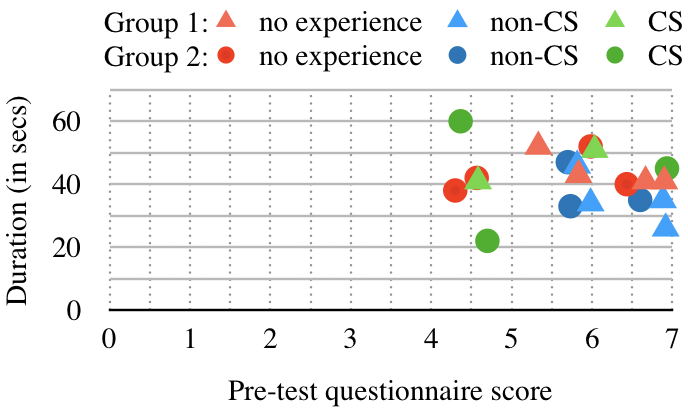
\includegraphics[width=\textwidth]{figures/quan-pretest-results.png}%
%     \caption{Pre-test vs Task duration}\label{fig:pretestvstask}%
%   \end{subfigure}~~%
%   \begin{subfigure}[h]{0.24\textwidth}%
%     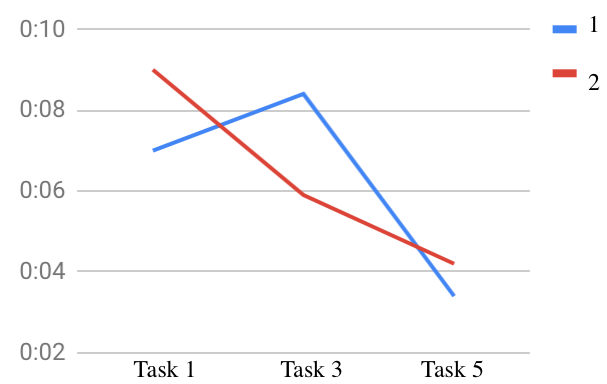
\includegraphics[width=\textwidth]{figures/quan-groups-duration.png}%
%     \caption{Task duration per group}\label{fig:taskvsgroup}%  
%   \end{subfigure}
%   \caption{}
%   \label{fig:task-duration}%
% \end{figure}%

% \begin{figure}[tp]
%   \subfigure[Pre-test vs Task duration]{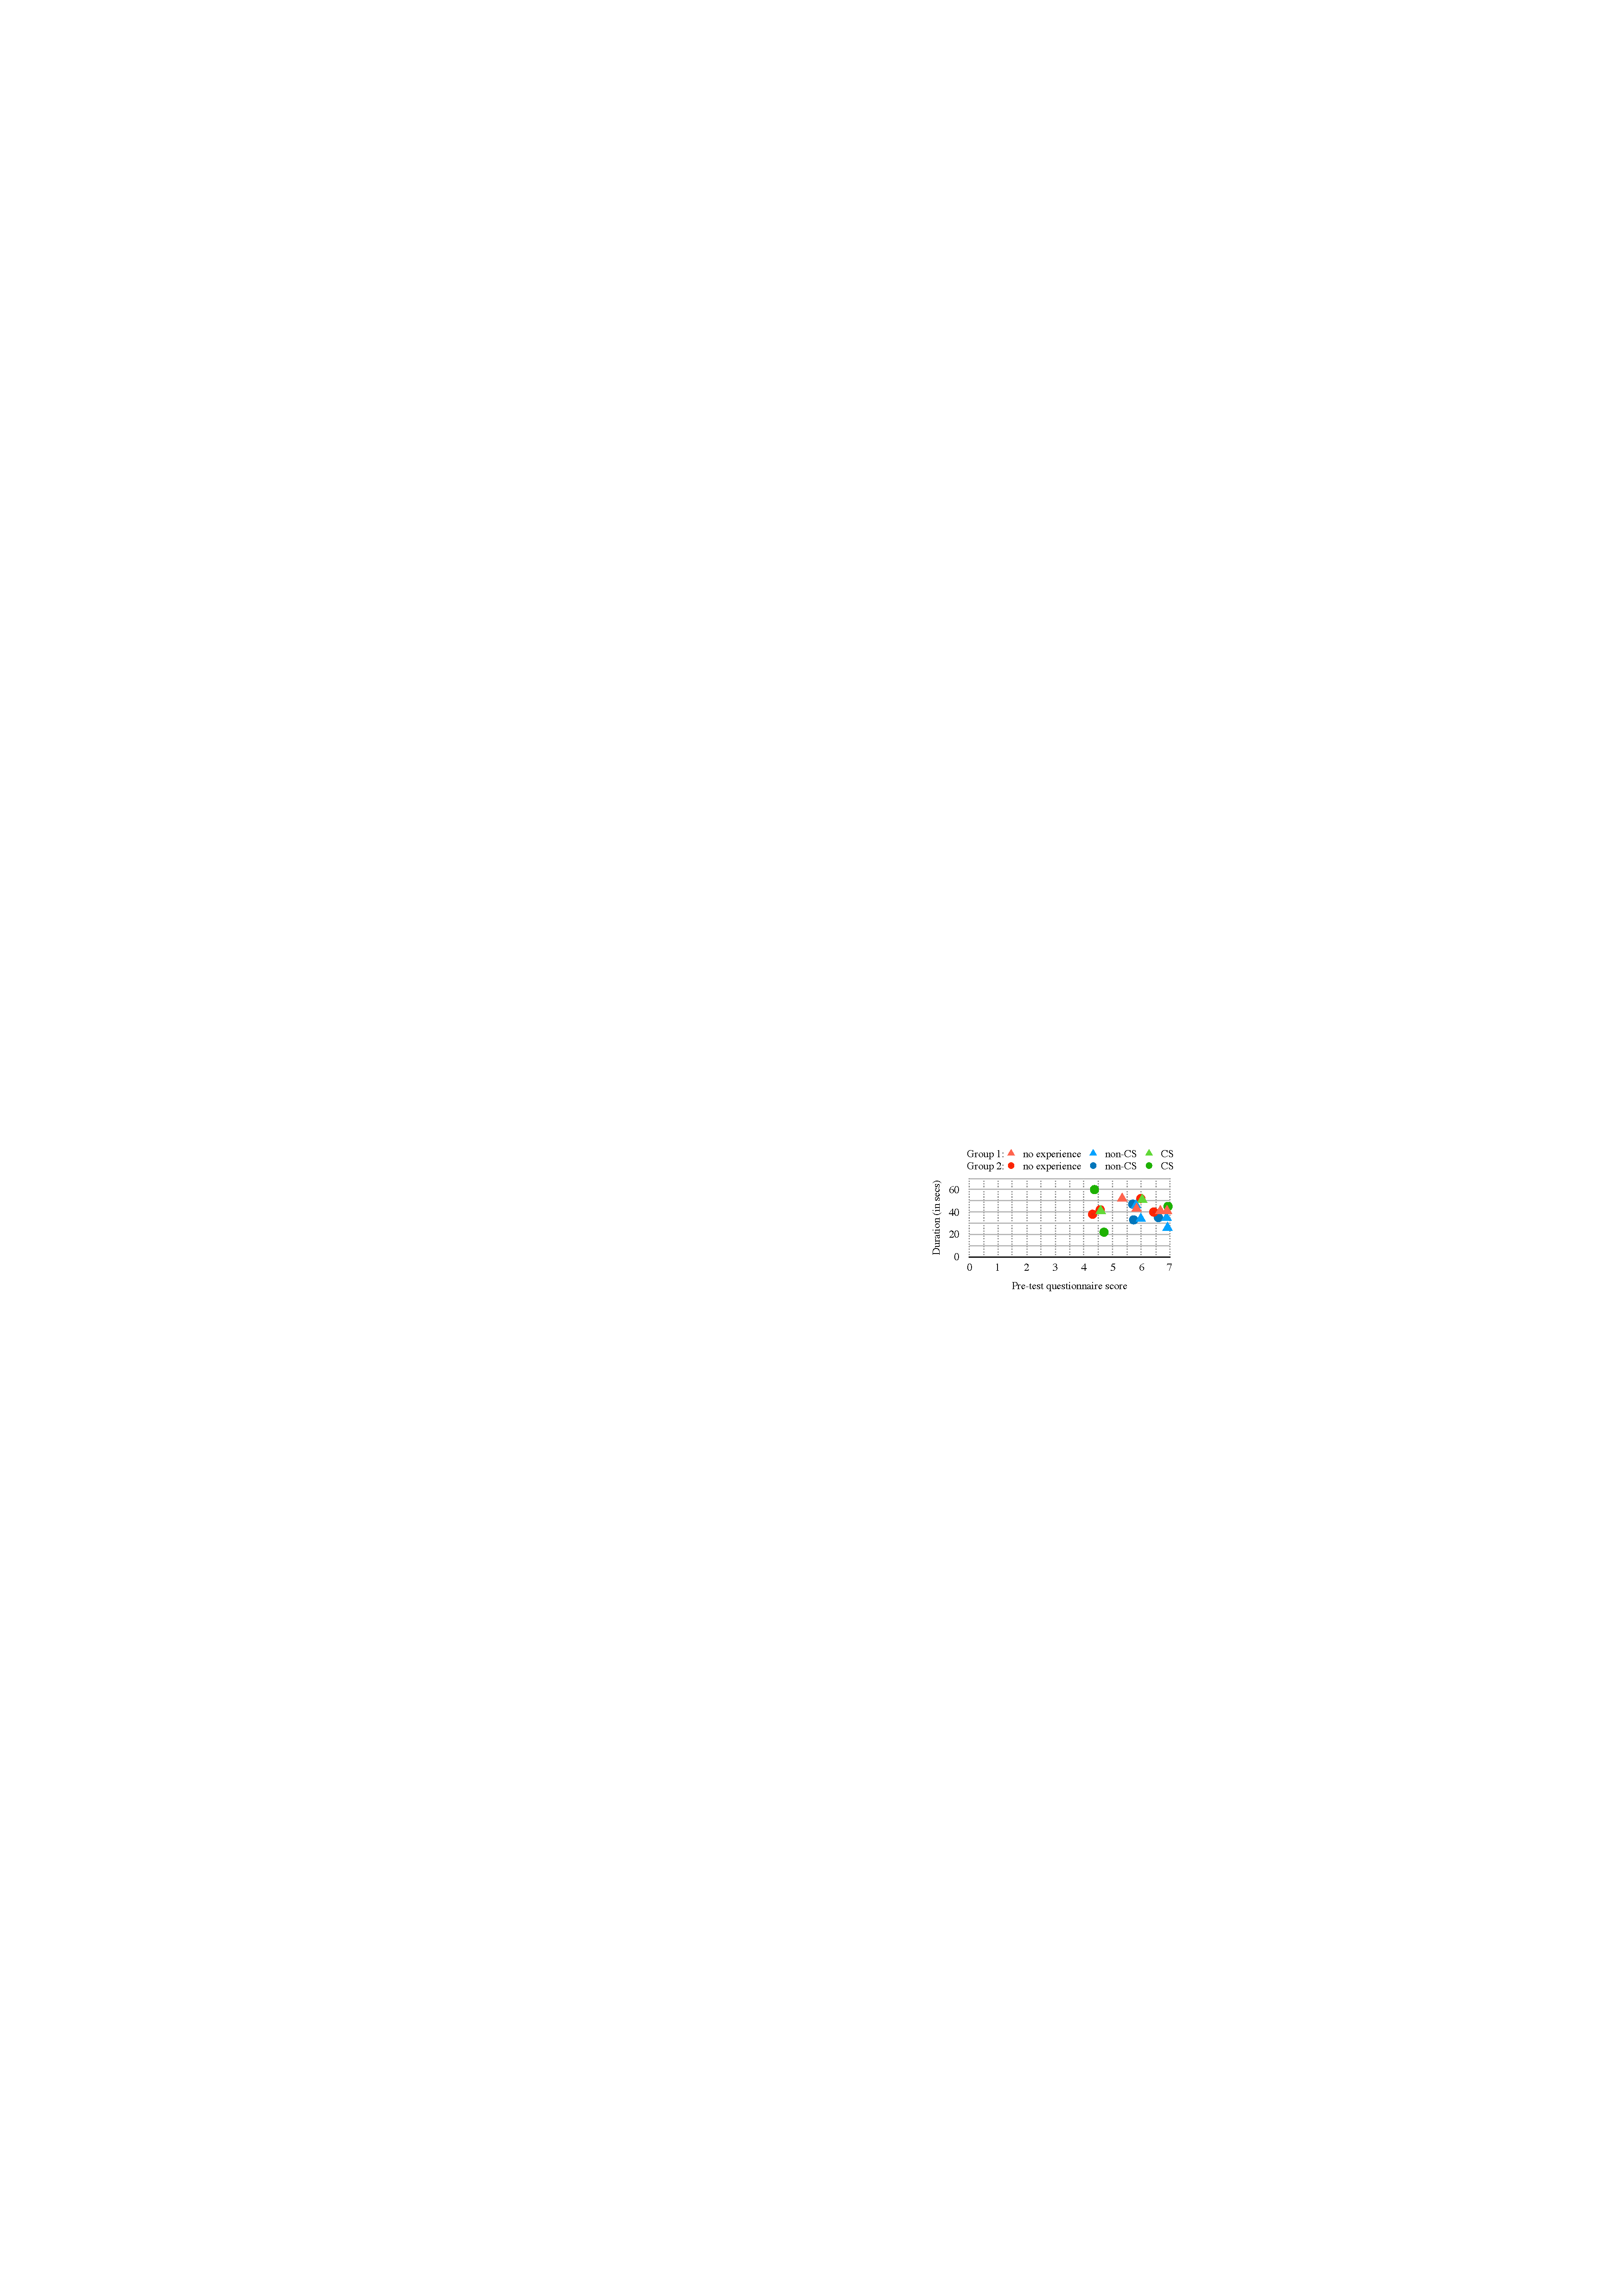
\includegraphics[width=0.48\linewidth]{figures/quan-pretest-results.pdf}}
% \label{fig:pretestvstask}\quad
%   \subfigure[Task duration per group]{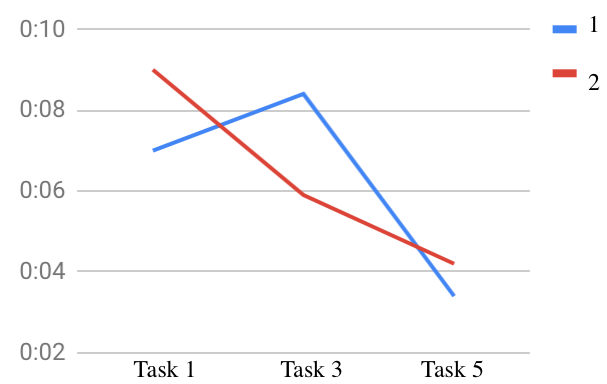
\includegraphics[width=0.48\linewidth]{figures/quan-groups-duration.png}}
% \label{fig:taskvsgroup}
% \end{figure}

\subsubsection*{Condition inference (H4)} 
To evaluate user programming strategies, the condition inference (CI) (see \sect{sec:inference}) in our study only generated a minimal set of predicates, which did not cover predicates needed for later tasks.
We noticed a discrepancy in the programming strategies between the two control groups (Group 1 with CI vs Group 2 without CI).
As participants in Group 2 had to add action conditions manually, they considered all predicates they deemed necessary for the action and therefore added additional ones that were required for later tasks.
On the other hand, we observed that Group 1 had the tendency to leave the inferred conditions unmodified without adding conditions that were missing.
%7/10 users in Group 1 did not modify the inferred conditions and did not put much thought potentially missing conditions.
Thus, Group 2 took on average longer to complete tasks where a new action had to be created (Tasks 1\&6), but was faster than Group 1 for subsequent tasks, where conditions had to be modified (Tasks 3,5,7).
Overall both groups had similar completion times for all tasks (Group 1: AVG=41, STD=7.89 and Group 2: AVG=41.4, STD=10.56).

\subsubsection*{Task duration vs Pre-test questionnaire (H5)} 
As expected, participants who demonstrated a better understanding of the introduced concepts in the pre-test questionnaire completed the main tasks (Tasks 3-8) faster on average (\fig{fig:pretestvstask}).
Users scored between 4.3-6.93 out of 7 points (AVG=5.8, SD=0.91), with task completion times between 22-60 minutes (AVG=41.2, SD=9.07).
`non-CS' users scored above average points (AVG=6.23, STD=0.55) and completed the fastest (AVG=36.6, STD=7.46).
As an outlier we observed that the fastest participant scored only 4.7, but easily learned how to use the system and completed the tasks in 22 minutes.
%the participant that took the longest (60min) scored 4.37.
Even though Group 1 performed slightly better in the pre-test (AVG=7.5, STD=1.35) than Group 2 (AVG=6.4, STD=2.01), both completion times were on average similar (41min).

\begin{figure}[h]%
	\centering
	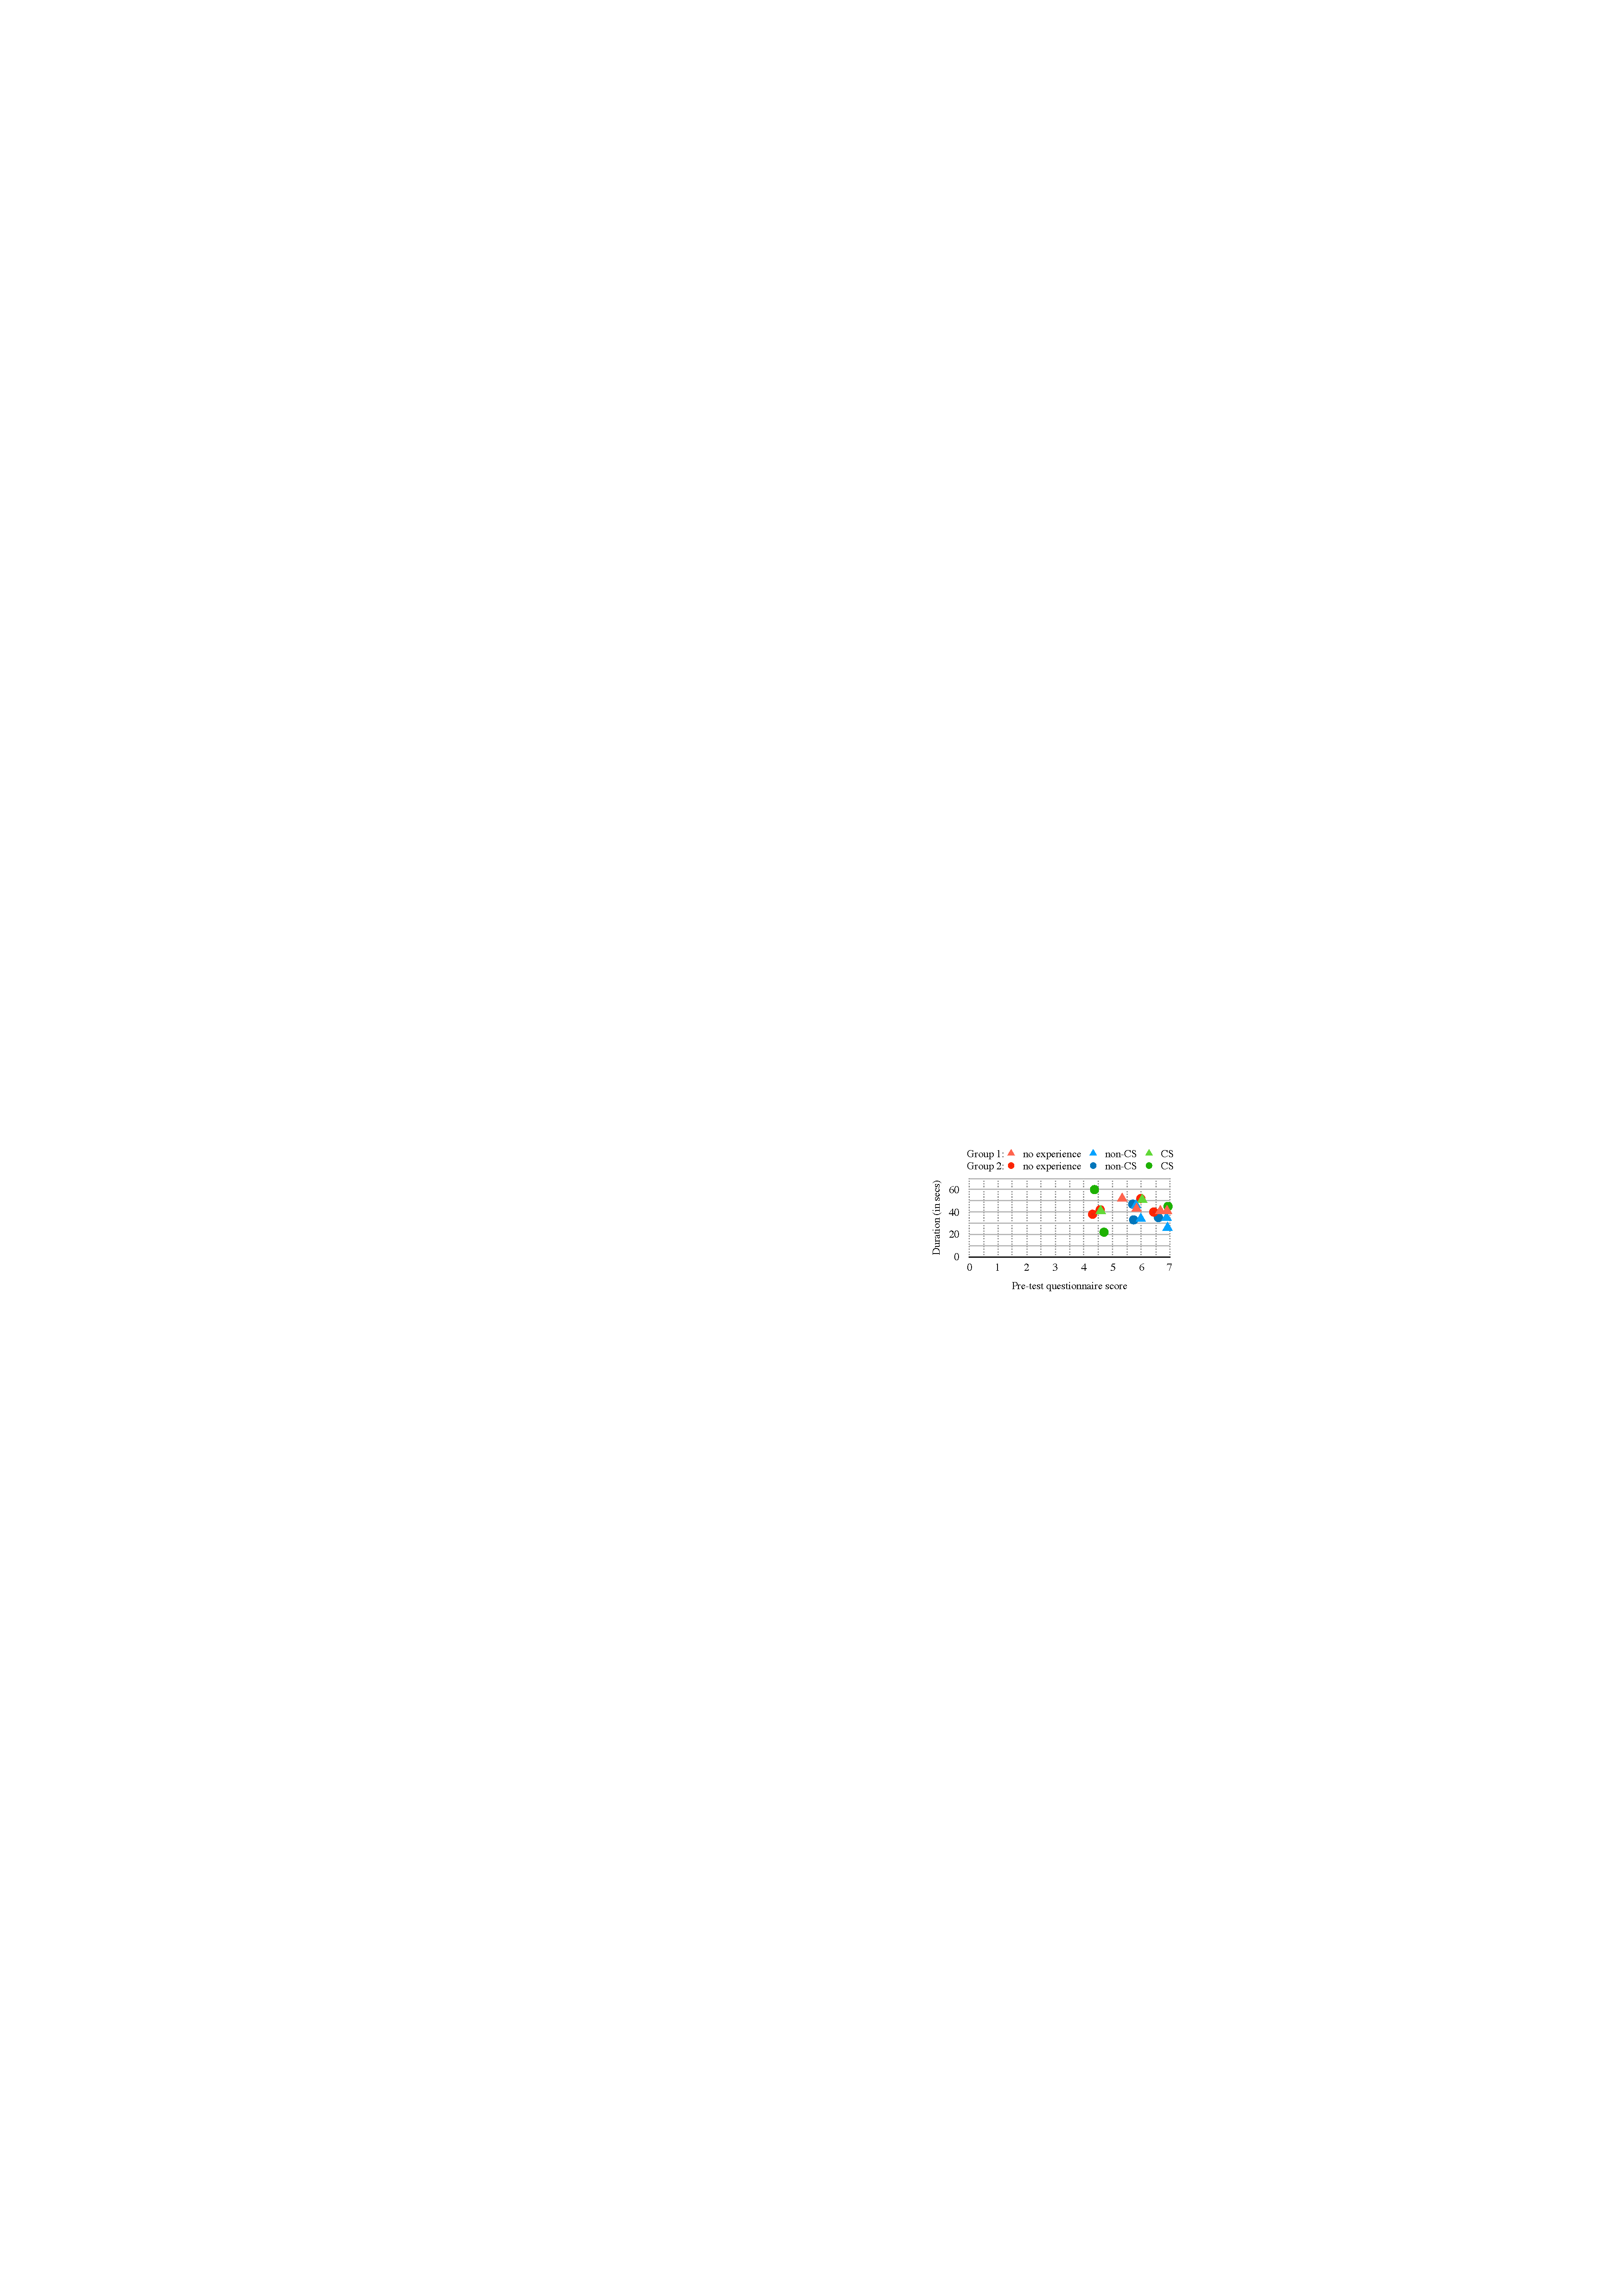
\includegraphics[width=0.6\columnwidth]{figures/quan-pretest-results.pdf}%
	\caption{Participants who did better in the pre-test questionnaire completed the main tasks faster, with `non-CS' users scoring the highest and being the fastest on average.}\label{fig:pretestvstask}%
\end{figure}%
%In Task 3: as all the users in Group 2 had added the missing condition (`posB is clear') in Task 1, a correct action sequence was generated directly.
%In Group 1 8/10 had not added this condition and needed guidance to resolve this issue, with 3 participants trying to modify the problem definition instead of the action, 1 trying to add a new action for `clearing a position', and 1 failing to figure out the right condition to add.


% \begin{table}[h]
% \centering
% \caption{TO DO: User performance with (Group 1) and without condition inference (Group 2) where Tasks 1 and 2 were training.}
% \label{table:performance}
% \begin{center}
% \begin{tabular}{ccc}
% Task & Group 1 & Group 2 \\ \hline
%  & Action/Problem & Action/Problem \\
% (1) & 0:30 () & 0:40 \\
% (2) & 0:30 & 0:40 \\ \hline
% 3 & 0:30 & 0:40 \\
% 4 & 0:30 & 0:40 \\
% 5 & 0:30 & 0:40 \\
% \hline
% %6 & (3,3,1) off-grid & Pick, place, push left\&front & Tin cans \\
% %7 & (3,3,1) off-grid & Pick, place, push left\&front& Soda cans \\
% %8 & (2,3,1) interleaving & Pick and place from top & Candy bags \\ 
% Total & 0:30 & 0:40 \\ \hline
% Pre-Test Score & 8/10 & 7/10 \\ 

% \end{tabular}
% \end{center}
% \end{table}

\subsubsection*{System usability and learnability} 
There are several ways to interpret the System Usability Scale (SUS) scores (\cite{brooke2013sus}) obtained from the post-study survey. 
Using \citet{bangor2008suseval} categories, 14 (70\%) users ranked iRoPro as `acceptable', 6 (30\%) rated it `marginally acceptable', and no one ranked it `not acceptable'.
Correlating this with the Net Promoter Score\footnote{https://measuringu.com/nps-sus/}, this corresponds to 10 (50\%) participants being `promoters' (most likely to recommend the system), 5 (25\%) `passive', and 5 (25\%) `detractors' (likely to discourage).
Overall, iRoPro was rated with a good system usability which has been shown to be correlated with its learnability (\cite{borsci2009dimensionality,sauro2011practical}).

\subsubsection*{User experience} 
%We asked users the same questions as in our previous work \textit{[Anonymous]} where we used the Wizard-of-Oz technique to conduct a qualitative evaluation of a potential system.
% similar with mainly positive responses in both studies .
Comparing the responses to the user study conducted in \sect{sec:Exp2}, where the Wizard-of-Oz technique was used to simulate the robot programming process, the main difference was regarding difficulties encountered during the experiment.
While in \sect{sec:Exp2} we had 11 (or 100\%) agree that they encountered no difficulties, only 7 (or 35\%) of our users in this study stated the same (\fig{fig:exp1vsexp2-results}).
However, all of our users claimed to have a good understanding of the action representation and how the robot learned new actions from the demonstration, while in the previous study, an average of 2 (18\%) disagreed.
Both differences can be explained by the fact that in our latest study, users had to use an end-to-end system to program the robot, while we previously simulated the system functionalities using the Wizard-of-Oz technique.
Even though our users encountered more difficulties, they got a better understanding of the functionalities due to getting hands-on experience.
This also correlates with negative responses in our survey to the question if `no programming experience was required' where 13/20 (65\%) agreed and 4 disagreed.
%3 out of the 4 who disagreed had at least taken a programming course before.
Overall, our user study with iRoPro received positive responses similar to our previous study.

Users stated the most useful feature as `generate solutions to defined goals automatically' (9 or 45\%), followed by `robot learns the action from my demonstration' (4 or 20\%) -- two main aspects of our approach.
A common feedback was that `it takes time to understand how the system works at the start'.
4 (20\%) stated that the most difficult part was `finding out why Baxter didn't solve a problem correctly', similarly 8 (40\%) stated difficulties related to `understanding predicates and defining conditions'. 
11 (55\%) disliked `assigning action conditions' the most, while the rest stated different aspects.
The most liked actions were `executing the generated plan' (8 or 40\%) and `demonstrating an action on Baxter' (7 or 35\%).
%Overall, users performed well in both control groups and gave positive feedback.

\begin{figure*}
	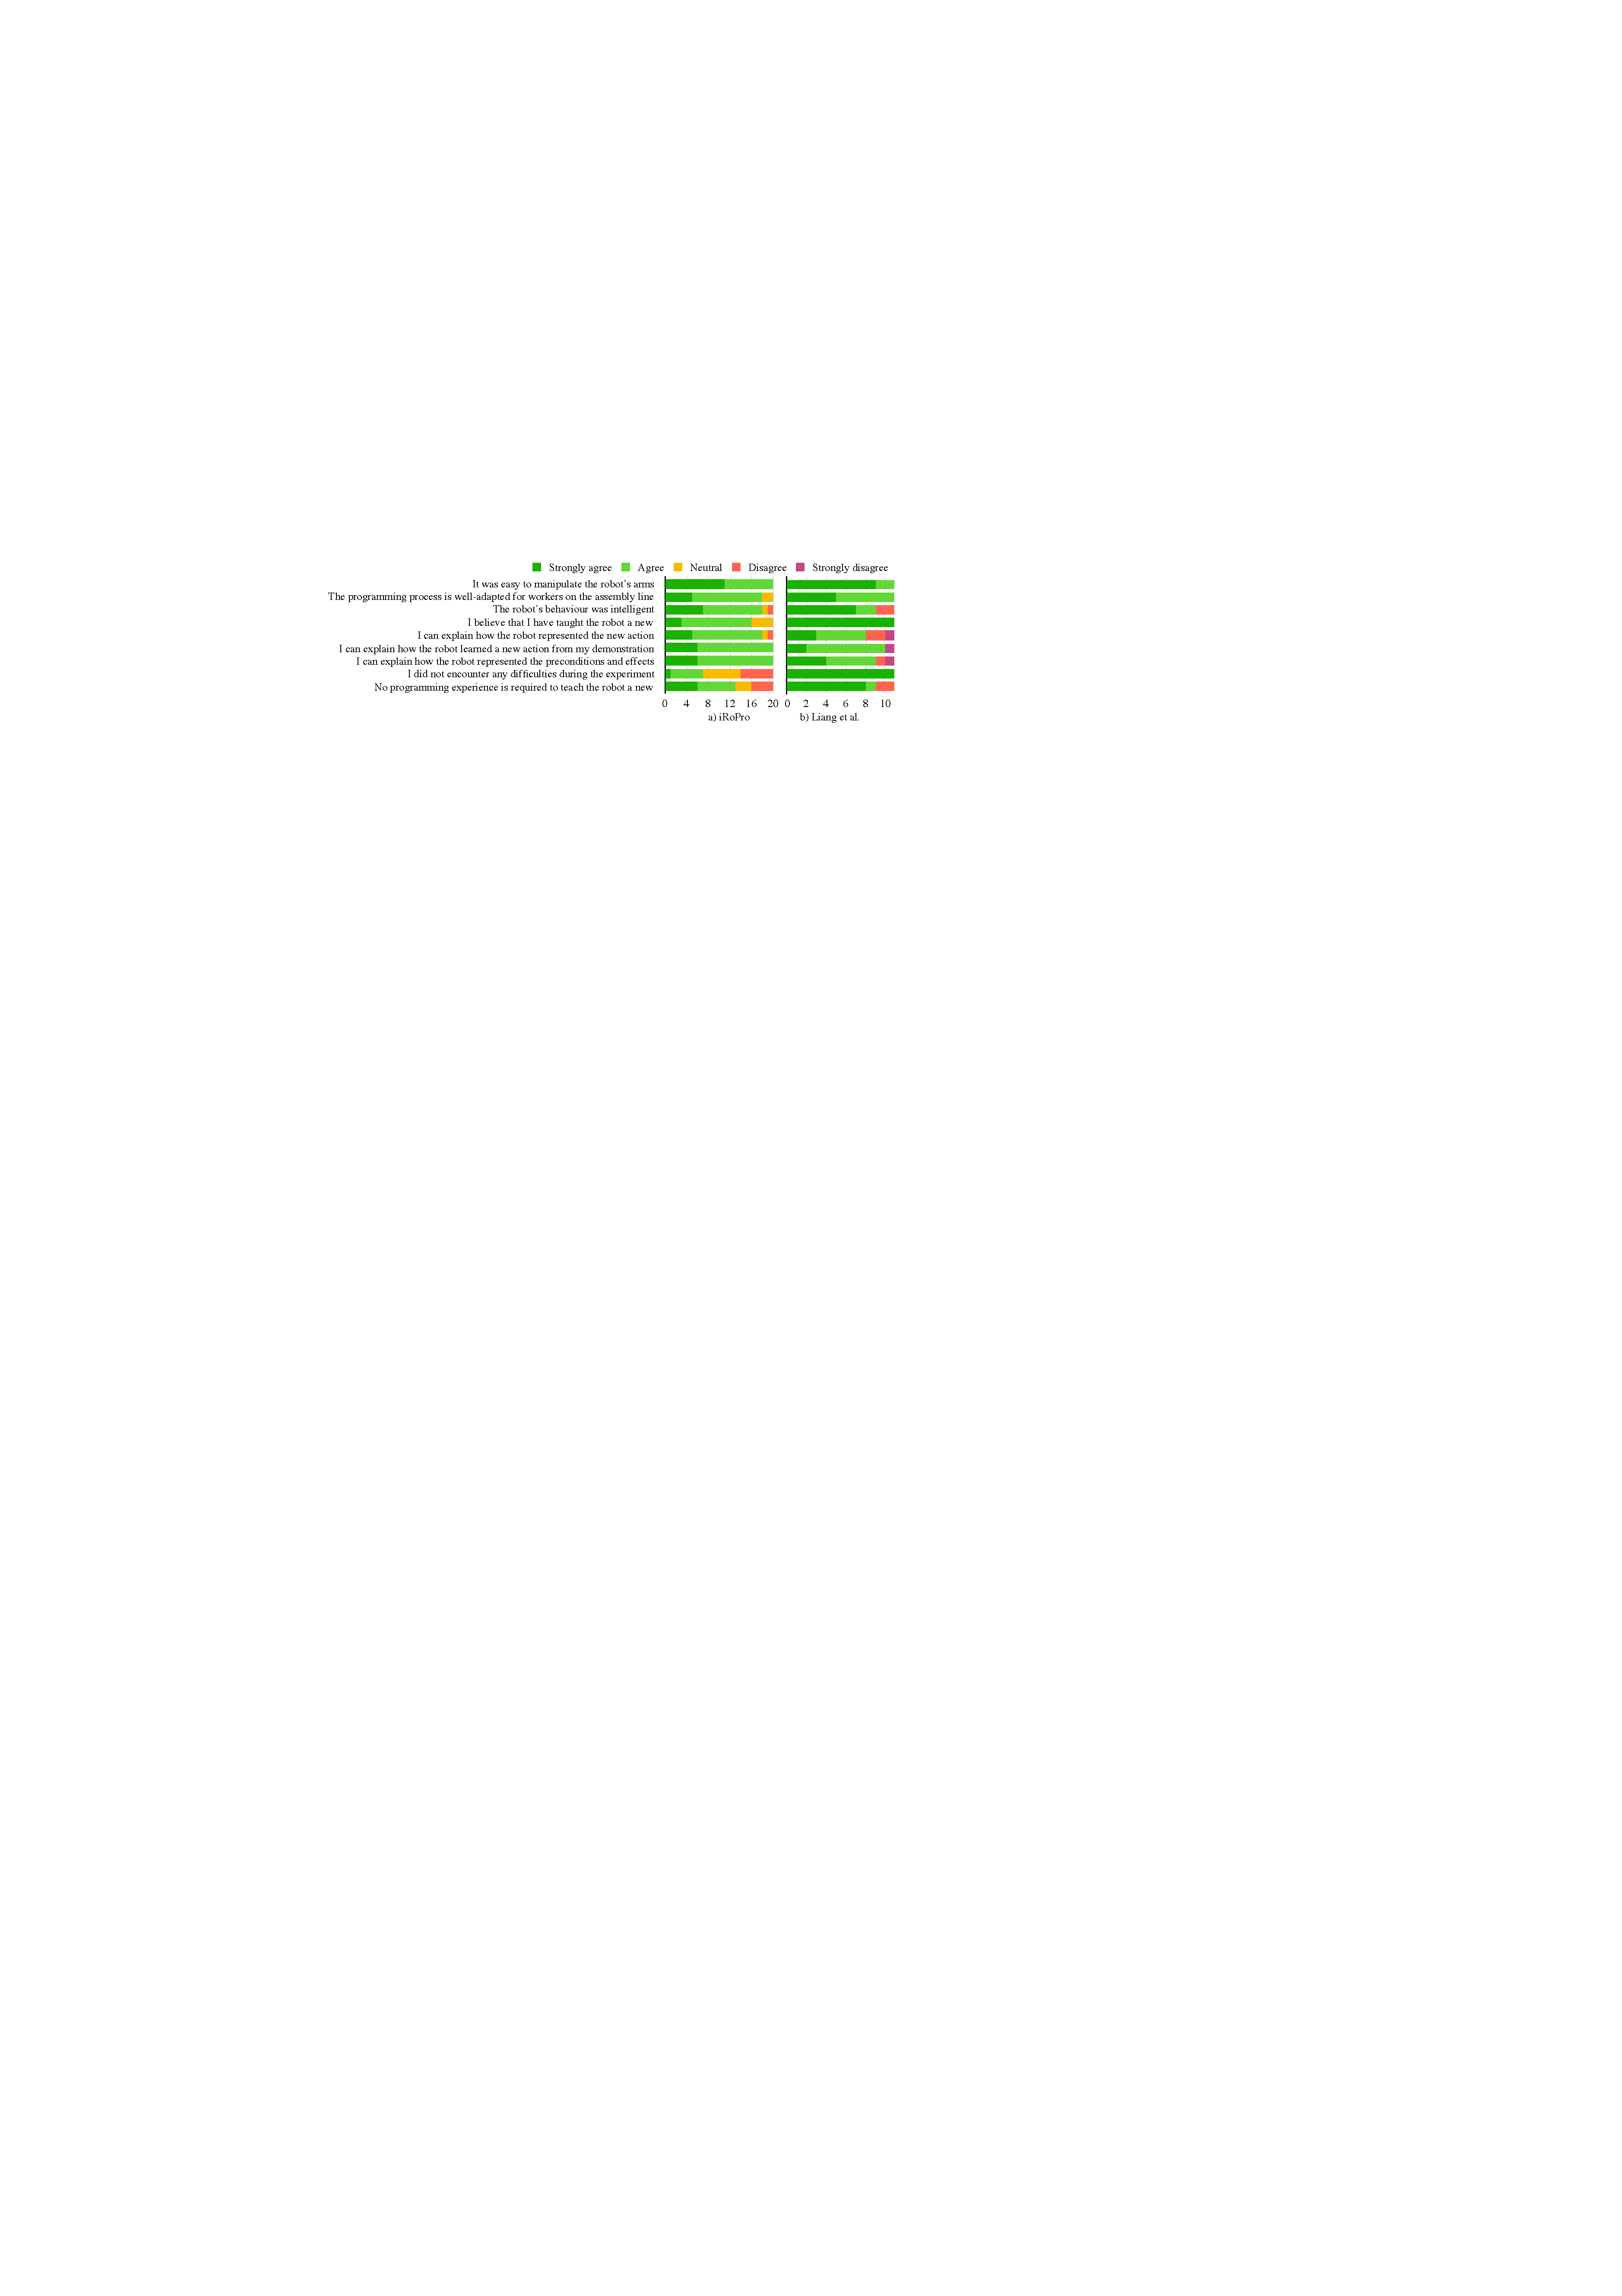
\includegraphics[width=0.98\linewidth]{figures/quan-exp1vsexp2-results.pdf}
	\caption{User responses from the post-study questionnaires comparing a) the iRoPro user evaluation (N=20) with responses obtained in b) the pre-experiment user study (N=11) (\sect{sec:Exp2}).}
	\label{fig:exp1vsexp2-results}
\end{figure*}
% \subsection{User strategies}
% As we have two control groups A (with condition inference) and B (without condition inference), we noticed two user strategies
% During the experiment, we noted the user's intended strategy to complete a task.

% \todo figure of people who tried the actions below:
% Teach new action
% Copy existing action
% Modify existing action

% \paragraph{User activity} 
% \todo {ignore some activity log at the end because of problems with executions} \\
% \todo {from Participant10 onwards, it keeps generating solutions for some reason}\\
% We logged the user activity on the interface at each button click to analyse the time spent on each task.

% The main activities 
% \todo {show graph of time spent at each option}

\subsection{Continuous Improvement of the System}
The system underwent four phases of improvement, allowing us to refine the system functionalities, graphical user interface, and user instruction methods.
The four phases consisted of the following:

\begin{enumerate}
	\item {Feedback from an expert in experimental evaluation of systems that involve human-machine interaction (Dr. Nadine Mandran):\\
		Based on the feedback we received on our initial prototype, we changed the flow for introducing the system to a novice user as it included a lot of new information (\eg Programming by demonstration and Automated planning concepts) that they were not familiar with.
		We also updated the questions in the pre-test questionnaire to include the same keywords (\ie predicate names) as used during the experiment to allow consistency and participants to familiarise themselves.
		%		We also decided to change the PbD part to a simple recording.
	}
	\item {Pre-tests with 3 users:\\
		We ran pre-tests with 3 users who have never seen the system before and further improved the experiment flow (\eg create an action for one object at a time).
		We also made the user interface more friendly to include Baxter icons (\fig{fig:baxter-icons}) and eyes that followed the robot's moving joint (\cite{baxtereyes}) on the robot's screen so that it seemed more human-like.
		We also noticed that troubleshooting incorrect actions seemed difficult for all users, so we included an option to review actions and goals which provides a summary of the created input and hints to guide the debugging steps.}
	\item {First experimental tests with 5 users with condition inference:\\
		After running the experiments with 5 users, we noticed that the majority did not bother modifying the inferred action conditions.
		This raised an interesting HRI question of whether users who were given automatically generated conditions would `blindly trust' them.
		Hence, we decided to create two experiment groups: with and without condition inference, where the first 5 participants belonged to the former.
		Participants in the latter group would need to manually enter all conditions via the interface. }
	\item {Final experimental tests with 16 users: \\
		The remaining users were divided into the two control groups so that we had an equal number of participants in both control groups, while also maintaining an even distribution of programming levels.
		The results of the overall 21 participants were used as the final evaluation of the system as discussed in the previous sections.
	}
\end{enumerate}

\begin{figure*}
	\centering
	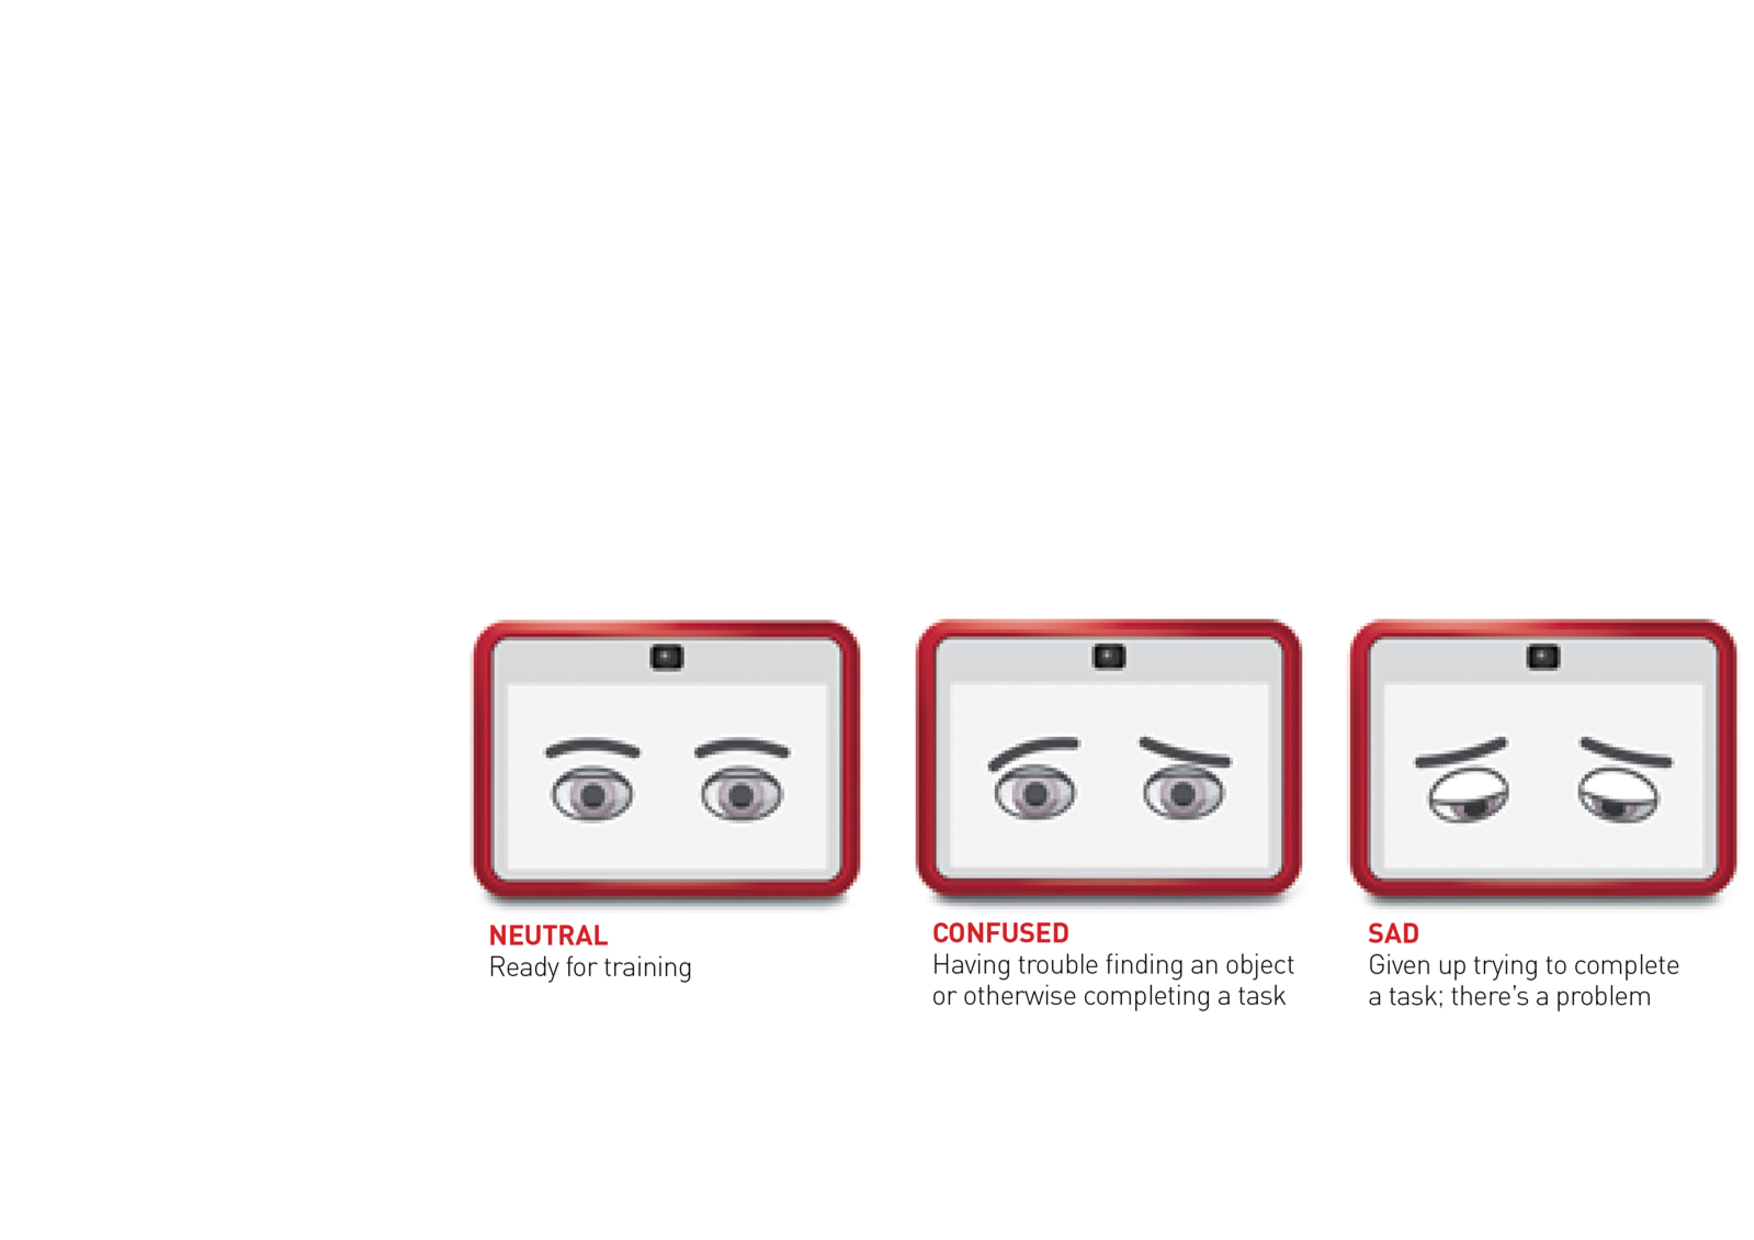
\includegraphics[width=0.8\linewidth]{figures/baxter-icons.pdf}
	\caption{Baxter icons used for the graphical interface (\cite{baxteremojis}).}
	\label{fig:baxter-icons}
\end{figure*}
%\begin{table}[h]
%	\centering
%	\caption{Continuous Improvement of the System}
%	\label{table:studyphases}
%	\begin{center}
%		\begin{tabular}{lll}
%			\#  & Evaluation & Improvements \\ \hline
%			1 & Initial prototype Feedback from Nadine Mandran & create new action (+demo) \\
%			2 & Pre-tests with 3 users & create new problem \\
%			3 & First experimental tests with 5 users & add condition (`is clear') \\
%			4 & Final experimental tests with remaining 15 users & modify types\\ \hline
%		\end{tabular}
%	\end{center}
%\end{table}

%In the following section we provide more details on the final two phases involving end-users.




\section{Discussions}
\label{sec:discussion}
Both system and user evaluations demonstrated that iRoPro can be used to generalise primitive actions to a range of complex manipulation tasks and that it is easy to learn for users with or without programming experience.
In our system evaluation we could have programmed other actions, such as turning or pushing for packaging tasks.
As the purpose of our evaluation was to show the generalisability of primitive actions with the use of a task planner, we decided to stick to pick-and-place actions.
%Users particularly liked the PbD technique and found that
%`generating plans automatically' was the most useful feature 
In the following we discuss limitations and interesting extensions of our work:
\begin{enumerate}
	%\item No generalization from one item to another.
	\item Our object perception is limited as it does not detect objects that are too close together (\eg stacked objects).
	An improved perception system would allow the detection of initial states with stacked objects, automatically detecting goal states, or verifying action executions.
	% TO DO: Could include limited gripper width, etc. as in tremblay2018synthetically
	%s mentioned in \sect{sec:implementation}, we partly the latter by using a mental model, where we first executed a stacking task to save the latest object positions, then reused the saved state for subsequent tasks.
	\item Due to the different grippers, we did not program actions that use both arms (\eg carrying a tray). A possible extension would be to include a better motion and task planning system in order to allow executing both arms simultaneously while avoiding self-collision.
	%As our robot was equipped with a suction and a claw gripper, the kinesthetic teaching of both arms could be difficult to program by a single user.
	\item We only included a minimal set of predicates (\sect{sec:highlevel}) that we deemed intuitive and useful for object manipulation tasks.
	It could be interesting to include and learn predicates to capture more complex domains such as object orientation (\cite{li2016learning}).
	%the use a mobile robot that can move between workstations.
	%\item A possible extension would be to incorporate probabilistic techniques to learn predicates or pre-train the robot on simulated scenarios to improve the condition inference.
\end{enumerate}

\section{Conclusion} 
\label{sec:conclusion}
In this chapter we presented iRoPro, an interactive Robot Programming system that allows simultaneous teaching of low- and high-level actions by demonstration.
The robot reuses the actions with a task planner to generate solutions to complex tasks that go beyond the demonstrated action.
The approach was implemented on a Baxter robot and we showed its generalisability on six benchmark tasks by teaching a minimal set of primitive actions that were reused for all tasks.
We further demonstrated its usability with a user study where participants with diverse educational backgrounds and programming levels learned how to use the system in less than an hour.
Both user performance and feedback confirmed iRoPro's usability, with the majority ranking it as `acceptable' and half being promoters.
Overall, we demonstrated that our approach allows users with any programming level to efficiently teach robots new actions that can be reused for complex tasks.
Thus, we enable end-users to program robots from scratch, without writing code, therefore maximising the generalisability of taught actions with minimum programming effort.